\documentclass[letterpaper,11pt]{article}

\usepackage{latexsym}
\usepackage[empty]{fullpage}
\usepackage{titlesec}
\usepackage{marvosym}
\usepackage[usenames,dvipsnames]{color}
\usepackage{verbatim}
\usepackage{enumitem}
\usepackage{hyperref}
\usepackage{fancyhdr}
% \usepackage{fontspec}
% \usepackage{xeCJK}
\usepackage{graphicx}
\usepackage[UTF8]{ctex}
\usepackage{blindtext}
\usepackage{multicol}
\usepackage{wrapfig}


% \setCJKmainfont{SimSun}

\pagestyle{fancy}
\fancyhf{} % clear all header and footer fields
\fancyfoot{}
\renewcommand{\headrulewidth}{0pt}
\renewcommand{\footrulewidth}{0pt}

% Adjust margins
\addtolength{\oddsidemargin}{-0.375in}
\addtolength{\evensidemargin}{-0.375in}
\addtolength{\textwidth}{1in}
\addtolength{\topmargin}{-.5in}
\addtolength{\textheight}{1.0in}

\urlstyle{same}

\raggedbottom
\raggedright
\setlength{\tabcolsep}{0in}

% Sections formatting
\titleformat{\section}{
  \vspace{-4pt}\scshape\raggedright\large
}{}{0em}{}[\color{black}\titlerule \vspace{-5pt}]

%-------------------------
% Custom commands
\newcommand{\resumeItem}[2]{
  \item\small{
    \textbf{#1}{: #2 \vspace{-2pt}}
  }
}

\newcommand{\resumeSubheading}[4]{
  \vspace{-1pt}\item
    \begin{tabular*}{0.97\textwidth}{l@{\extracolsep{\fill}}r}
      \textbf{#1} & #2 \\
      \textit{\small#3} & \textit{\small #4} \\
    \end{tabular*}\vspace{-5pt}
}

\newcommand{\resumeSubItem}[2]{\resumeItem{#1}{#2}\vspace{-4pt}}

\renewcommand{\labelitemii}{$\circ$}

\newcommand{\resumeSubHeadingListStart}{\begin{itemize}[leftmargin=*]}
\newcommand{\resumeSubHeadingListEnd}{\end{itemize}}
\newcommand{\resumeItemListStart}{\begin{itemize}}
\newcommand{\resumeItemListEnd}{\end{itemize}\vspace{-5pt}}




\begin{document}


%----------HEADING-----------------
% \begin{tabular*}{\textwidth}{l@{\extracolsep{\fill}}r@{\extracolsep{0pt}}}
%   \textbf{\href{https://accle123.github.io/}{\Large 杨淇 }} \\
%   Mobile : 178-4227-3879 \\
%   Email : \href{mailto:yangqi2568@gmail.com}{yangqi2568@gmail.com} \\
%   Blog :\href{https://accle123.github.io/}{https://accle123.github.io} \\
%   Github : \href{https://github.com/ACCLE123?tab=stars}{https://github.com/ACCLE123?tab=stars} \\
%   Acwing : \href{https://www.acwing.com/user/myspace/index/134003/}{https://www.acwing.com/user/myspace/index/134003/} \\
%   Leetcode :\href{https://leetcode.cn/u/yang-qi-ar/}{https://leetcode.cn/u/yang-qi-ar/} \\
% \end{tabular*}

\noindent
\begin{minipage}{0.8\textwidth}
\textbf{\href{https://accle123.github.io/}{\Large 杨淇 }} \\
  Mobile : 178-4227-3879 \\
  Email : \href{mailto:yangqi2568@gmail.com}{yangqi2568@gmail.com} \\
  Blog :\href{https://accle123.github.io/}{https://accle123.github.io} \\
  Github : \href{https://github.com/ACCLE123?tab=stars}{https://github.com/ACCLE123?tab=stars} \\
  Acwing : \href{https://www.acwing.com/user/myspace/index/134003/}{https://www.acwing.com/user/myspace/index/134003/} \\
  Leetcode :\href{https://leetcode.cn/u/yang-qi-ar/}{https://leetcode.cn/u/yang-qi-ar/} \\
\end{minipage}%
\begin{minipage}{0.2\textwidth}
  \centering
  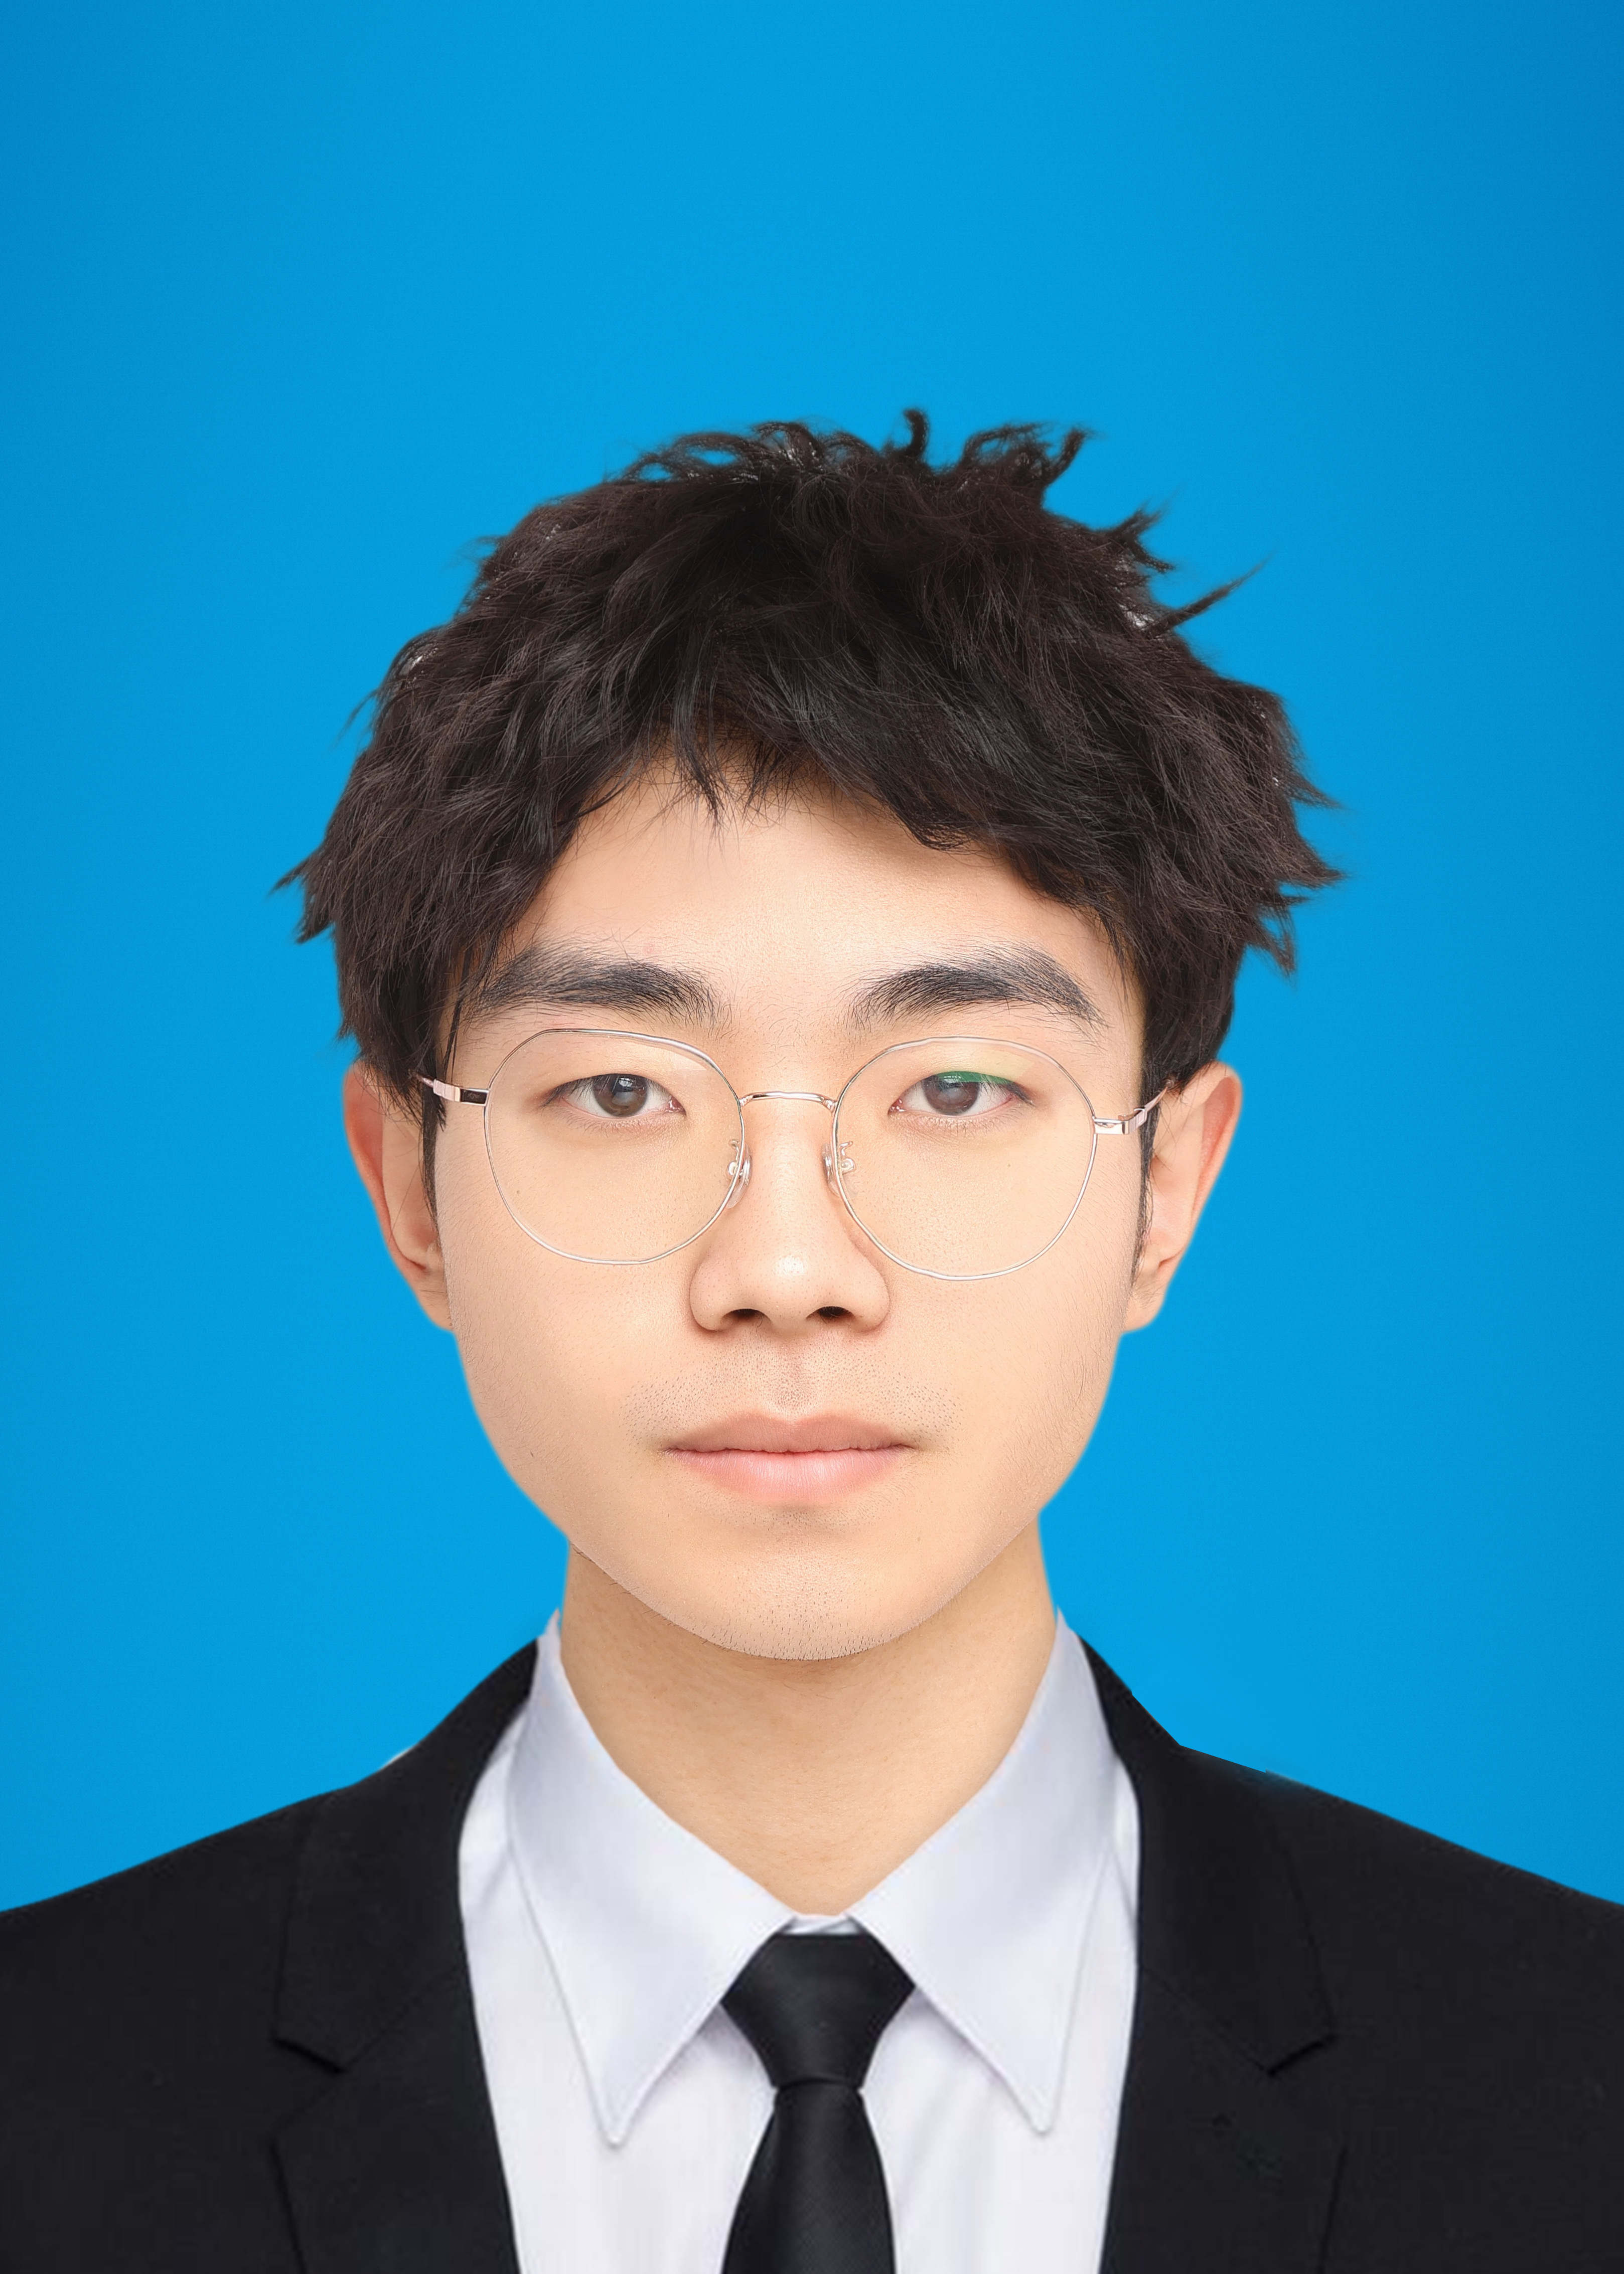
\includegraphics[width=2.5cm]{yangqi.JPG}
\end{minipage}



%-----------EDUCATION-----------------
\section{Education}
  \resumeSubHeadingListStart
    \resumeSubheading
      {南开大学}{本科}
      {计算机科学与技术}{Sep. 2021 -- Present}
  \resumeSubHeadingListEnd

%-----------HONORS AND AWARDS-----------------
\section{Honors and Awards}
  \resumeSubHeadingListStart
    \resumeSubItem{校级学业奖学金}
      {获得南开大学颁发的校级学业优秀奖学金,表彰在本科学习期间的优异表现。}
    \resumeSubItem{全国数学建模省级一等奖}
      {大三上学期,参加数学建模获得省级一等奖}
    \resumeSubItem{PAT甲级70分}
      {在大一参加PAT,获得70/100分}
  \resumeSubHeadingListEnd

%-----------PERSONAL STRENGTHS-----------------
\section{Personal Strengths}
    \resumeSubHeadingListStart
    \resumeSubItem
       {算法}
      {长时间学习算法,并在leetcode,acwing等平台进行大量学习刷题。} 
    \resumeSubItem{开源}
      {经常游览github,热爱开源平台,长时间使用过ubuntu作为工作时使用的操作系统} 
    \resumeSubItem{运动}
      {大一参加过计算机学院足球比赛,习惯健身,有良好的抗压能力}
    \resumeSubItem{学习}
      {喜欢底层,喜欢新技术,有很强的学习能力,擅长使用google+gpt4进行快速学习,有较强适应能力}
  \resumeSubHeadingListEnd


%-----------EXPERIENCE-----------------
\section{Experience}
  \resumeSubHeadingListStart

    \resumeSubheading
      {天清数安科技有限公司}{天津}
      {后端实习生}{Jan. 2024 to Apr. 2024}
      \resumeItemListStart
        \resumeItem{智慧养老项目}
          {设计数据库,使用springboot搭建后端,完成员工模块、老人注册模块、服务模块。项目基于ruoyi进行二次开发。}
        \resumeItem{游泳溺水检测项目}
          {使用yolov8,使用python进行摄像头对接,主要负责警报系统、处理视频展示的业务。完成初步版本,并在服务器上进行部署。}
      \resumeItemListEnd

  \resumeSubHeadingListEnd

%--------PROGRAMMING SKILLS------------
\section{Programming Skills}
 \resumeSubHeadingListStart
     \resumeItem{Languages}{: Python, Javascript, C++, SQL, Java} 
     \resumeItem{Technologies}{: SpringBoot, JVM, Linux, MySQL, PostgreSQL, Redis, Docker, Git, Vuejs, REST}
 \resumeSubHeadingListEnd


%-----------PROJECTS-----------------
\section{Projects}
  \resumeSubHeadingListStart
    \resumeSubItem{buzhi校园平台 }
      {校园社交平台,完成发帖子,多级评论,点赞,收藏,消息提醒的接口}
    \resumeSubItem{my-mini-spring}
      {正在进行,该项目为学习项目,为了提高自己对spring核心原理的认识,通过阅读mini-spring和spring源码进行学习。}
    \resumeSubItem{my-db}
      {正在进行,该项目为学习项目,是简单的c语言实现的数据库,目前完成了table(hard code), pager,statement部分。可以进行插入和查询操作}
    \resumeSubItem{xv6}
      {正在进行,该项目为学习项目,xv6是mit os作业, 目前完成到lab4 虚拟内存部分。项目为risc-v下到简易操作系统。}
  \resumeSubHeadingListEnd

%



%-------------------------------------------
\end{document}
